\label{partie_architecture}
L'application est conçue selon le \textit{modèle en couche}, bien qu'elles ne soient pas strictes.
Elle n'utilise \underline{pas} le pattern MVC
\footnote{\label{MVC_pas_utile}Pattern pour les applications disposant de vue.
  Les dépendances ne sont pas les mêmes que pour le modèle en couche}.
L'architecture globale est expliquée dans cette section, les paquetages sont un peu plus détaillées ensuite si nécessaire.

\begin{figure}[!h]
  \centering
  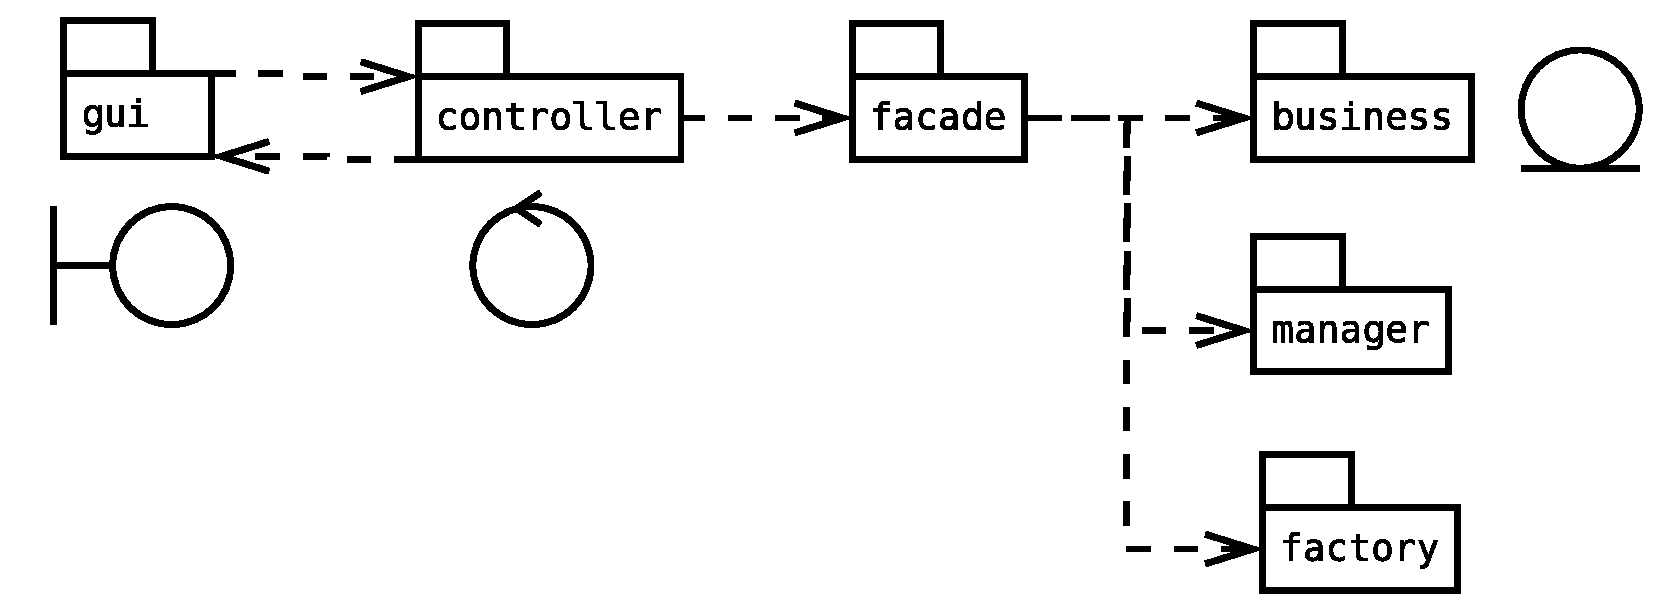
\includegraphics[width=14cm]{images/paquetage.eps}
  \caption{Diagramme de paquetage de l'application.}
  \label{diagramme_de_paquetage_idb}
\end{figure}

\subsection{Couche présentation}
La couche \textit{présentation} contient les IHM de l'application.
Le code des classes ne contient que ce qui est nécéssaire pour l'agencement et le paramétrage des composants sur la vue.

Sur la figure \ref{diagramme_de_paquetage_idb}, la couche présentation se trouve dans le paquetage \textit{gui} (Graphic User Interface, IHM en français).

\subsection{Couche contrôle}
La couche \textit{contrôle} contient l'\textit{intelligence} des IHM, c'est à dire ce qu'il doit se passer \textbf{hors} de la vue (dans les bases de données, la RAM etc.) après un clic sur tel ou tel bouton, case à cocher ou tout autre composant.

Cette couche décharge le code des IHM et fait office d'\textit{indirection} entre les vues et le reste de l'application : les IHM ne connaissent que leurs contrôleurs respectifs.

Sur la figure \ref{diagramme_de_paquetage_idb}, la couche contrôle se trouve dans le paquetage \textit{controller}.
Comme le montre le diagramme, les dépendances entre les paquetages \textit{gui} et \textit{controller} ne sont pas unilatérales.
C'est trompeur : en réalité, les contrôleurs connaissent leurs IHM uniquement pour éviter de les afficher en double.
Il était possible de faire des IHM des \textit{singletons}, cependant cela n'aurait pas réglé le défaut du \textit{fort couplage}.

Les IHM ne sont donc pas des singletons et les contrôleurs y sont associés (au sens UML du terme).

\subsection{Couche entité}
La couche \textit{entité} ou \textit{métier} contient la valeur ajouté de l'application, c'est à dire toutes les classes qui offrent le service proposé par l'application.

Dans ce projet tuteuré, les classes métiers sont une pseudo-couche \gls{orm}
\footnote{\label{faux_orm}Les ORM convertissent les données en objets, dans cette application se sont les \textit{conteneurs} des données qui sont convertits en objets.}
qui représentent les tables et les contraintes du SGBD connecté à l'application.
Elles limitent les accès au SGBD, ce qui augmente les performances de l'application et participent à la génération de code SQL à partir des saisies faites dans les IHM.

Sur la figure \ref{diagramme_de_paquetage_idb}, la couche métier se trouve dans le paquetage \textit{business}.

\subsection{Couche facade}
La couche \textit{facade} reprend le \textit{design pattern} façade.
Son utilité est de limiter les dépendances entre les contrôleurs et les autres couches de l'application. Elles n'apportent rien d'autres à l'application.

Sur la figure \ref{diagramme_de_paquetage_idb}, la couche facade se trouve dans le paquetage \textit{facade}.

\subsection{Couche DAO}
La couche \gls{dao} permet d'enregistrer et récupérer des informations depuis le SGBD.
En temps normal, les DAO permettent d'enregistrer des données.
Dans cette application, ils permettent d'enregistrer les données, leurs conteneurs (tables) et les \glspl{constraint}.
Ils ont également un rôle de générateur de SQL, généralement "simple" et qui diffère selon le SGBD connecté, contrairement aux classes métiers qui fournissent du SQL qui fonctionne sur tous les SGBD.

Sur la figure \ref{diagramme_de_paquetage_idb}, la couche DAO se trouve dans le paquetage \textit{manager}.
Les DAO sont utilisés \textit{à peu près} en suivant le design pattern \textit{data mapper}
\footnote{\label{faux_data_mapper}Ce pattern stipule que ce soient les classes qui \underline{utilisent} les \gls{orm} qui les enregistrent dans un système de stockage.}
, dans le sens où ce sont les contrôleurs de l'application qui les utilisent (par le biais des façades) pour enregistrer les tables.

\subsection{Couche fabriques}
L'une des problématique de ce projet est de faire fonctionner l'application par dessus tous les SGBD disponibles.
Bien que le langage SQL soit normé, les SGBD ne l'implémentent pas de la même manière, ce qui veut dire qu'il est \underline{différent} d'un SGBD à l'autre. C'est la difficulté principale pour que l'application fonctionne sur tous les SGBD. Il y a d'autres difficultés mais elles sont mineures, comme la gestion de la casse
\footnote{\label{casse_et_sgbd}Oracle convertit le nom des tables et contraintes en majuscule, ce qui n'est pas le cas de MySQL par exemple.}.

Cela prend beaucoup trop de temps de faire un code qui fonctionne pour tous les SGBD.
Ce n'est pas ce que l'application propose.
Elle ne fonctionne qu'avec les SGBD Oracle et MySQL.
En revanche, elle est conçue pour s'adapter à un nouvel SGBD sans modifier le code existant (ou presque), il "suffit" d'en ajouter pour utiliser un nouvel SGBD.

Pour cela, l'application utilise une \textit{fabrique abstraite}.

Sur la figure \ref{diagramme_de_paquetage_idb}, la fabrique se trouve dans le paquetage \textit{factory}.
Les dépendances de ce paquetage ne sont pas toutes représentées sur la figure.
Ce qui est visible dans le diagramme c'est que la fabrique est toujours appelée depuis un contrôleur (lui-même passant par les façades).
En plus de cela, la fabrique possède des dépendances de stéréotypes \textit{create} vers les paquetages :
\begin{itemize}
\item \textbf{gui} : \underline{pas} pour fabriquer des IHM, mais des classes imposées par Java pour les faire fonctionner, avec un comportement différent selon le SGBD connecté.
\item \textbf{manager} : pour créer des DAO générant le code SQL adapté au SGBD connecté.
\end{itemize}
